
\section{Chiến lược bao phủ đa robot với đội hình chữ V}
\label{sec:sea}
Phương pháp RCPP gồm ba bước như sau:\\

\subsection{Tìm các cặp cạnh đối đỉnh}
Các cặp đối đỉnh là các cặp đỉnh của đa giác mà cho phép các đường hỗ trợ song song giao với ranh giới của đa giác và nằm hoàn toàn về một phía của nó. Chúng có thể được xác định bằng thuật toán của Shamon \cite{shamos1978computational}\\

Ở phần này, vấn đề sẽ được giải quyết từ góc độ 2D, do đó không gian làm việc sẽ là không gian hai chiều và nó sẽ được gọi là máy bay. Một điểm trên không gian làm việc được xác định bởi một cặp giá trị $(x, y)$. Cho rằng vùng quan tâm (ROI) là mặt phẳng, vì vậy nó được biểu thị bằng một hình dạng lồi dạng tiêu chuẩn (convext) \cite{10.1007/11841036_57}, $Q = \{ V, E \}$. Trong đó $V$ là tập hợp các đỉnh, điểm trong cùng một mặt phẳng đặt theo chiều kim đồng hồ. $E$ là tập hợp các cạnh tạo bởi 2 điểm liên kết nhau.

Ta sẽ định nghĩa đường hỗ trợ là một đường thẳng đi qua 1 đỉnh của đa giác hoặc 1 cạnh của đa giác và nằm hoàn toàn về một phía của đa giác, không cắt đa giác tại điểm nào. Một cặp điểm đối đỉnh là 1 cặp điểm mà ở 2 điểm đó tồn tại 2 đường hỗ trợ đi qua và song song với nhau và khoảng cách giữa 2 đường thẳng song song chính là chiều rộng của đa giác

Nhiệm vụ khảo sát được thực hiện bởi một máy bay không người lái mang một máy ảnh đang chiếu xuống mặt đất như hình \ref{fig:FOVmodel}. Giả sử sử rằng Robot được xác định là một điểm $P = (X, Y)$, trong đó X và Y là tọa độ NED. Khi máy bay không người lái bao phủ một khu vực, nó cất cánh tại điểm PS, di chuyển đến khu vực quan tâm, đi theo một con đường trong khi nó chụp ảnh và cuối cùng di chuyển đến điểm hạ cánh, PE . Hiện tại một bức tranh được chụp, máy ảnh có thể chụp được một hình chữ nhật trên mặt đất.

Đường kính của hình đa giác lồi là khoảng cách lớn nhất giữa các đường hỗ trợ song song. Tham khảo Hình \ref{fig:anh1} và lưu ý rằng các đường hỗ trợ song song không thể được thực hiện để vượt qua từng cặp điểm. Ví dụ, không có đường hỗ trợ nào đi qua các đỉnh D và F có thể song song với nhau. Điều này có nghĩa là DF không phải là đường kính. Một cặp điểm tồn tại các đường hỗ trợ song song sẽ được gọi là cặp đối đỉnh. Vì vậy chúng ta chỉ cần xem xét các cặp đối đỉnh. Vấn đề là tìm thấy chúng mà không kiểm tra tất cả các cặp điểm

    \begin{figure}[H]
        \centering
        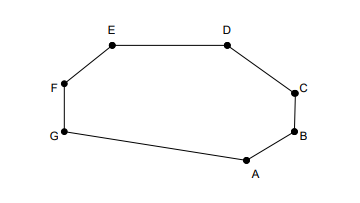
\includegraphics[width=0.7\textwidth]{chapter4/image/anh1.png}
        \caption{Hình Polygon}
        \label{fig:anh1}
    \end{figure}

\subsubsection{Phương pháp tìm cặp điểm đối đỉnh}
$\bullet$ Quá trình thứ 1: Quay theo cùng chiều kim đồng hồ:
Bây giờ đề cập đến Hình \ref{fig:anh2}, quan sát rằng các dòng L và N là các đường hỗ trợ song song thông qua các đỉnh A và D, tương ứng. Điều này có nghĩa là (A,D) là một cặp đối đỉnh nhau. Khi ta bắt đầu tiến hành quay đường hỗ trợ đồng thời theo chiều kim đồng hồ về các đỉnh này, chúng vẫn là các đường hỗ trợ. Điều này vẫn đúng cho đến khi một trong các đường hỗ trợ trở nên trùng hợp với một cạnh của đa giác. Ở đây L, khi được xoay vào vị trí L', sẽ chạm vào cạnh DE trước khi N đến B. Vì vậy (A, E) trở thành một cặp đối đỉnh. Tiếp tục theo cách này, chắc chắn sẽ tìm ra được tất cả các cặp chống đối, vì các đường song song sẽ di chuyển qua tất cả các góc có thể. Xác định cặp mới ở mỗi bước chỉ liên quan đến một so sánh góc đơn giản.
    \begin{figure}[H]
        \centering
        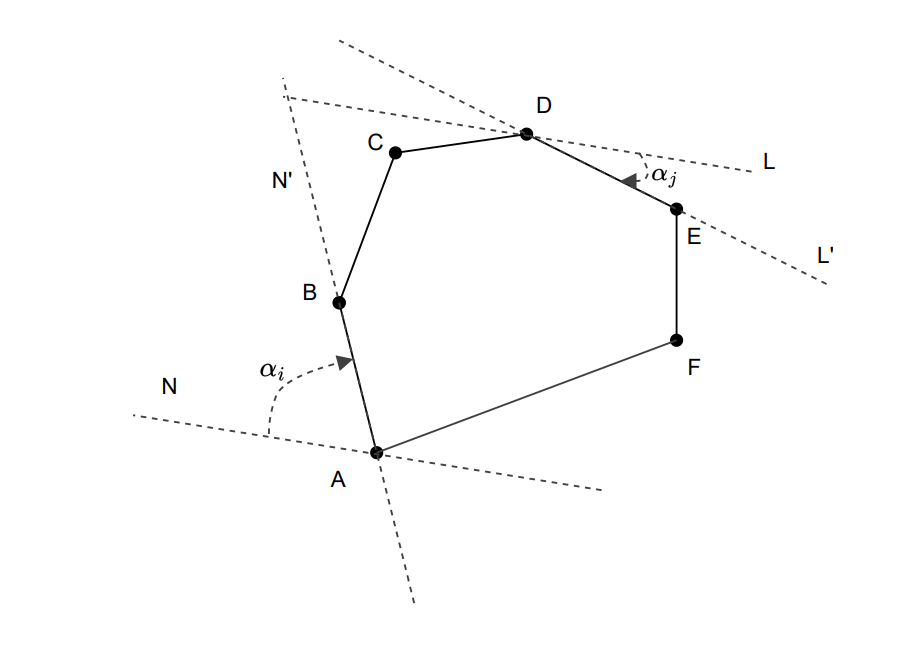
\includegraphics[width=0.7\textwidth]{chapter4/image/anh2.png}
        \caption{Xác định cặp đối đỉnh theo chiều thuận kim đồng hồ}
        \label{fig:anh2}
    \end{figure}

 Từ hình \ref{fig:anh3}, bằng cách tìm góc tối thiểu giữa $\alpha_{i}$ và $\alpha_{j}$, là các góc từ các đường hỗ trợ ảo đến cạnh gần nhất của đa giác theo thuận chiều kim đồng hồ. Tuy nhiên, thay vì đo $\alpha_{i}$ và $\alpha_{j}$, thuật toán đã đo sự khác biệt giữa vòng quay từ dòng L đến N. Xem các dòng 1-8 của Thuật toán \ref{alg:Findpoint}.Nhìn hình\ref{fig:anh3} ta có thể thấy nếu sự khác biệt giữa 2 góc $\gamma$  trừ $\pi$ nhỏ hơn 0 thì cạnh DE được lấy làm cơ sở của đường dẫn. Mặt khác, nếu sự khác biệt giữa 2 góc $\gamma$  trừ $\pi$ lớn hơn 0,  cạnh AB được lấy làm đế của cạnh. Một trường hợp đặc biệt là khi cả hai góc đều bằng nhau. Trong trường hợp như vậy, số lượng đường đi là như nhau sau đó, nó không quan trọng đường cơ sở nào được chọn theo số lượng đường đi. Vì lý do này và sự đơn giản trong thuật toán, trong trường hợp các góc bằng nhau, thuật toán sẽ chọn cạnh AB làm cơ sở
    \begin{figure}[H]
        \centering
        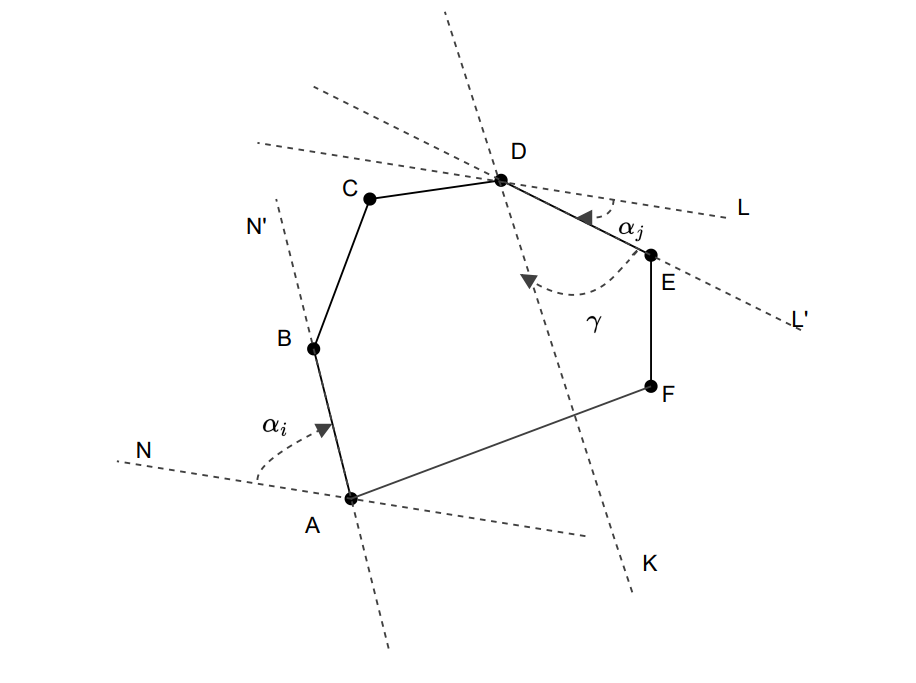
\includegraphics[width=0.7\textwidth]{chapter4/image/anh3.png}
        \caption{Xác định sự khác biệt giữa 2 góc theo chiều thuận kim đồng hồ}
        \label{fig:anh3}
    \end{figure}

$\bullet$ Quá trình thứ 2: Quay ngược chiều kim đồng hồ:
Trong bước này, có một vài trường hợp tìm thấy đường cơ sở khác bằng cách xoay caliper theo hướng ngược chiều kim đồng hồ.  Các góc đối với đường thẳng B(đường thẳng được tạo bởi 2 điểm C,D) sẽ được đo. Các góc đo $\gamma_{B}$, góc giữa CE với đường thẳng B và $\gamma_{A}$, là góc giữa cạnh LN với đường thẳng song song với B.  Đối với đường thẳng A, một đường thẳng hỗ trợ song song với đường thẳng B  đi qua L được cho là đỉnh đối với C. Một góc bổ sung $\phi$ cần có để đường thẳng A có thể chạm được đến cạnh LM. Vì đường thẳng B đã được chạm vào DC  trước A , do đó $\phi$ góc lớn hơn hoặc bằng không.
Các góc $\gamma_{A}$ và $\gamma_{B}$ sẽ cho chúng ta biết gần nhất cạnh cơ sở  từ hai khả năng: CD hoặc LM sẽ là đường cơ sở. Xem dòng 9-19 từ Thuật toán \ref{alg:Findpoint}.
    \begin{figure}[h]
        \centering
        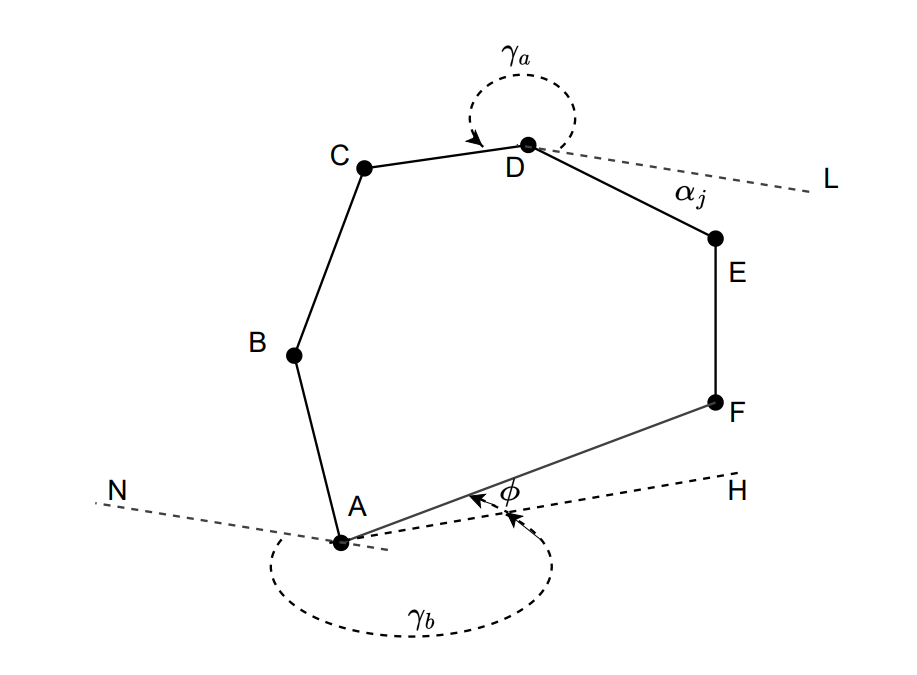
\includegraphics[width=0.7\textwidth]{chapter4/image/anh4.png}
        \caption{Xác định cặp đối đỉnh theo chiều ngược kim đồng hồ}
        \label{fig:anh3}
    \end{figure}

Phương pháp trên có thể tóm gọn thông qua Thuật toán \ref{alg:Findpoint} như sau: \\

\begin{algorithm}
% \SetKwComment{Comment}{/* }{ */}
\KwData{:\textbf{V} = \{1,2,...n\} và các cặp đối đỉnh (i,j)}
\KwResult{$\rho$}
{
\tcc*[h]{Quay theo chiều thuận kim đồng hồ}\\
\If{($\text{angle}(i,j)-\pi < 0$)} 
{
    $b \gets j$\;
    $a \gets i$\;
}   
\Else
{
    $b \gets i$\;
    $a \gets j$\;
}
 \tcc*[h]{Quay ngược chiều kim đồng hồ}\\
$\phi \gets angle(b,a)-\pi $\\
$\gamma_{b} \gets angle(b-1,b) $\\
$\gamma_{a} \gets angle(a-1,a) - \phi $\\
    \If{$\gamma_{b} < \gamma_{a}$ }
    {
        $b_{2} \gets b-1$\\
        $a_{2} \gets a$
    }  
    \Else
    {
        $b_{2} \gets a-1$\\
        $a_{2} \gets b$
    }
}
\caption{Tìm kiếm các cặp điểm đối đỉnh}
\label{alg:Findpoint} 
\end{algorithm}

